\section{Implementation}
\label{Implementation}

In this section will be presented simple $C\#$ program as an example implementation of presented topics.
By design it implements the simplest multilayer network with two inputs and one output to model boolean functions.
Program is capable to learn non linearly separable XOR function and show this process.

\subsection{User interface}
\label{UserInterface}

User interface presents the network structure.

\begin{figure}[!h]
    \centering
    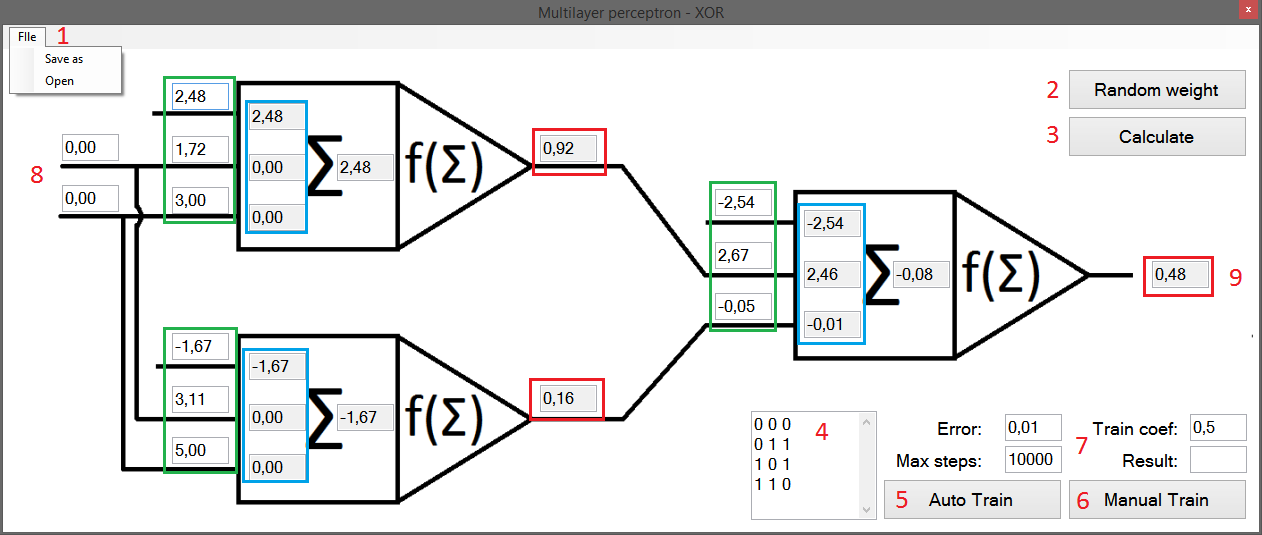
\includegraphics[scale=0.45]{Media/UI_numbers.png}
    \caption{User interface}
    \label{fig:UI}
\end{figure}

Elements of interface:
\begin{enumerate}[topsep=8pt,itemsep=-1ex,partopsep=1ex,parsep=1ex]
    \item \label{FileMenu} File menu - save and open network configuration with training data
    \item \label{RandomWeight} Random weight - set random values for neurons weights
    \item Calculate - calculate network output for given input values (8)
    \item \label{TrainingData} Training data - first two values are network inputs third value is desired network output
    \item \label{AutoTrain} Auto train - train network using given Training data
    \item Manual train - perform one iteration of \hyperref[formula:EBP]{EBP algorith} with given input (8) and output given in Result field (7) as training data
    \item Training parameters:
    \begin{enumerate}[topsep=-1ex,itemsep=-1ex,partopsep=1ex,parsep=1ex]
        \item \label{Error} Error - desired error value for Auto training (5)
        \item \label{MaxSteps} Max steps - limits number of Auto training iterations
        \item \label{TrainCoef} Train coef - corresponds to \textit{learn factor} $\alpha$
        \item Result - desired network output value for Manual training
    \end{enumerate}
    \item Network inputs - used for Manual training (6) and for manual network output calculation (3)
    \item Network output - calculated when button Calculate is pressed (3)
\end{enumerate}

\textcolor{ForestGreen}{\textbf{Green}} elements are neurons weights, \textcolor{Cerulean}{\textbf{blue}} are multiplication of weights and inputs, \textcolor{red}{\textbf{red}} are neurons outputs.

\subsection{Program structure}
\label{ProgramStrucutre}

Whole project is accessible on \url{https://github.com/gabr/kisem_xor} \\
It is based on two classes \textit{XORForm} and \textit{Network}:

\begin{itemize}[topsep=1pt,itemsep=-1ex,partopsep=1ex,parsep=1ex]
    \item \textit{XORForm}:
    \begin{itemize}[topsep=0pt,itemsep=-1ex,partopsep=1ex,parsep=1ex]
        \item Implements \hyperref[UserInterface]{User interface} actions
        \item Contains \textit{Network} class 
    \end{itemize}
    \item \textit{Network}:
    \begin{itemize}[topsep=0pt,itemsep=-1ex,partopsep=1ex,parsep=1ex]
        \item Contains all neurons weights $w$, inputs $u$ and it sum of weighted inputs~$S$
        \item Properties \textit{Inputs} and \textit{Output} gives access to \hyperref[InputLayer]{first} and \hyperref[OutputLayer]{last} layer of network
        \item \textit{\_connections} is a list of tuples where one tuple represents one connection between neurons
        \item \textit{\_rand} is a object used to generate random values of weights
        \item Methods implements \hyperref[UserInterface]{User interface} actions and the \textit{Train()} method implements \hyperref[formula:EBP]{EBP algorith}
    \end{itemize}
\end{itemize}

Whole classes structure can be seen on \hyperref[fig:Classes]{Figure \ref{fig:Classes}}.

\begin{figure}[!h]
    \centering
    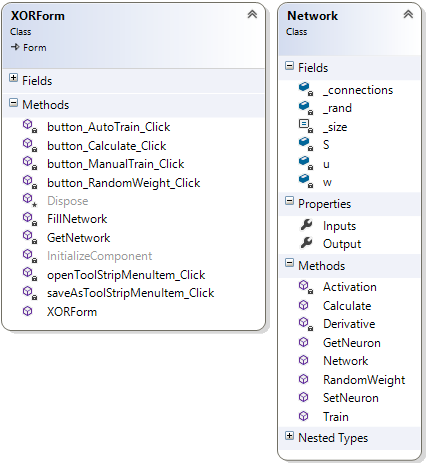
\includegraphics[scale=1]{Media/Class.png}
    \caption{Classes}
    \label{fig:Classes}
\end{figure}

\newpage

\subsection{Usage}
\label{Usage}

Usage of program on example of training boolean function XOR:
\begin{enumerate}[topsep=8pt,itemsep=-1ex,partopsep=1ex,parsep=1ex]
    \item \hyperref[UserInterface]{Open program}
    \item Set \hyperref[RandomWeight]{random weights}
    \item Provide true table for XOR function in \hyperref[TrainingData]{training data} window
    \item Set desired \hyperref[Error]{error} value and \hyperref[MaxSteps]{maximum iterations} value
    \item Set \hyperref[TrainCoef]{learning factor}
    \item Press \hyperref[AutoTrain]{Auto Train} button
\end{enumerate}

The resulted calculated weights can be saved using \hyperref[FileMenu]{File menu} \textit{File $\rightarrow$ Save as}.